\documentclass{amia}
\usepackage{graphicx}
\usepackage{subcaption}
\usepackage[labelfont=bf]{caption}
\usepackage[nomove]{cite}
\usepackage{color}
\usepackage[hidelinks]{hyperref}

\begin{document}

\title{Team20-Chest X-ray Pathology Detection with CNN}

\author{Xiao-Hong Deng$^{1}$, Gerry Meixiong$^{1}$, Chenxu Wen$^{1}$, Lan Yao$^{1}$}

\institutes{
	$^1$Georgia Institute of Technology, Atlanta, Georgia, USA \\
}

\maketitle

\noindent{\bf Abstract}


\textit{This project uses a convolutional neural network to reproduce the model presented in {\color{cyan}\cite{rajpurkar}}. We train and fine-tune the model on the CheXpert dataset provided by  {\color{cyan}\cite{irvin}}. The model is a multi-label image classifier that is able to predict and localize thoracic pathologies in X-ray images. We achieve performance comparable to the one presented in the original paper with a single model.} 

\section{Project Links}

Our project presentation slides are available \href{https://docs.google.com/presentation/d/1kbBUnL0xJCGYGuFPxePkkE4tbhmbp3xkT1xigkvserI/edit}{here}.

Our video presentation is available \href{https://www.youtube.com/watch?v=Tq4i1p9fv9s}{here} or at the following link: https://www.youtube.com/watch?v=Tq4i1p9fv9s

The code is available on GitHub \href{https://github.com/Xiaohong-Deng/6250Spring2020Team20Project}{here}.

\section{Introduction}
The chest X-ray is one of the most commonly accessible and effective radiological examinations for screening and diagnosis of many serious diseases in the United States. For example, more than 1 million adults are hospitalized with pneumonia and around 50,000 die from the disease in US every year according to CDC, 2017 and the chest X-ray is the best available method for diagnosing pneumonia.

However, even if chest X-ray is relatively cheap and can be performed with minimal procedural steps, detecting diseases such as pneumonia using chest X-ray is often challenging even for expert radiologists, and the availability of expert radiologists is very limited. Therefore, computer-aided diagnosis of diseases from chest X-rays with high-precision would not only have tremendous benefit in clinical settings, it would also be invaluable in delivery of health care to populations with inadequate access to diagnostic imaging specialists.



\section{Related Work}


In order to apply the rapidly developing techniques from deep learning and computer vision in the detection of diseases using chest X-ray, we will need lots of data.  One large public accessible chest X-ray dataset, "ChestX-ray14", was presented by {\color{cyan}\cite{wang}}. The dataset contains more than $100,000$ frontal-view X-ray images from over $30,000$ unique patients and it also comes with 14 disease image labels from associated radiological reports via natural language processing. The authors also  provided a unified weakly supervised multi-label image classification and disease localization framework to detect and spatially locate those diseases.  Another large dataset which is accessible by public, "CheXpert", which contains 224,316 chest (frontal and lateral views) radiographs of 65,240 patients labeled for the presence of 14 common chest radiographic observations, was presented by {\color{cyan}\cite{irvin}}.  The authors also investigated different approaches towards incorporating the uncertain labels into training convolutional neural networks.

{\color{cyan}\cite{Li2019}} presented an approach to perform disease identification and localization with a small number of location annotations. Their method involves first applying CNN to learn the entire image and then slicing the image into patch grid to learn the local information of the disease. 


{\color{cyan}\cite{rajpurkar}} developed an algorithm, CheXNet, a 121-layer Dense Convolutional Network (DenseNet) on the ChestX-ray14 dataset which can detect all 14 thoracic diseases at state-of-art level. Notably, CheXNet exceeds average radiologist performance on the F1 metric for pneumonia.

Many of the pathologies in lung X-ray are similar visually, and in general we have overwhelming normal samples v.s. disease samples in medical domain (imbalance data). In order to address those challenges, {\color{cyan}\cite{ge}} proposed a novel error function based on softmax concept (Multi-label Softmax Loss, MSML) and designed a convolutional deep network based on fine-grained classification methodology that incorporates MSML. They were able to improve the performance on the ChestX-ray14 compared to existing methods.


{\color{cyan}\cite{yao}} introduced an approach by applying a novel architecture that learns at multiple resolutions while generating saliency maps with weak supervision. They also parameterized the Log-Sum-Exp pooling function with a learnable lower-bounded adaptation (LSE-LBA) to build in a sharpness prior and better handle localizing abnormalities of different sizes using only image-level labels. They were able to set the state of the art on 9 diseases on ChestX-ray14 while generating saliency maps with high resolution.

{\color{cyan}\cite{gundel}} proposed a novel approach based on location-aware Dense Networks (DNetLoc), whereby they incorporate both high-resolution image data and spatial information for abnormality classification. They were able to obtain the best average AUC score on ChestX-ray14 dataset.

{\color{cyan}\cite{liu}} presented a method called segmentation-based deep fusion network (SDFN), to address potential drawbacks from existing methods caused by noise from misalignment and existence of irrelevant objects in the entire image, and by information loss from the resizing operation. They were able to improve the results of Gündel et al {\color{cyan}\cite{gundel}}.

Class activation maps has been proved to be reliable in localization task, which helps in locating the areas that may be related to the diseases in X-Ray images. {\color{cyan}\cite{zhou}} found that the CNN has remarkable localization ability without using any bounding box annotations. Weakly supervised object localization on the ILSVRC benchmark was conducted, and the result shows that the global average pooling CNNs can perform accurate object localization. Some other features of CAM are also discovered in their research. For example, the experiment of fine-grained classification was conducted and the result indicates that GoogLeNet-GAP with CAM can successfully localize and classify the objects. The ability of pattern discovery beyond objects is also demonstrated in the research.


\section{Dataset Description and Statistics}

In this project, we will use the CheXpert dataset {\color{cyan}\cite{irvin}}. CheXpert is a large public dataset for chest radiograph interpretation, consisting of 224,316 chest radiographs of 65,240 patients labeled for the presence of 14 observations as positive, negative, or uncertain. Each sample consists of a frontal-view image and a lateral-view image. It provides a version of the dataset with high image resolution and a downscaled version which is easier to work with.

The radiographic images and their associated radiology reports were collected from Stanford Hospital, between October 2002 and July 2017. 14 observations are chosen as labels based on the prevalence in the reports and clinical relevance. Most of the observations are pathologies with a few exceptions:
\begin{itemize}

	\item  No Finding: If there is no pathology labeled as positive or uncertain, give 1 to this observation. 
	\item  Pneumonia: Overall diagnosis.
	\item Support Devices: Observation that is not a pathology.
\end{itemize}



The training data was processed by an automatic labeler. The labeler extracted observation mentions from the associated radiology reports. After mentions were extracted, there were three stages in the labeling process: pre-negation, negation, and post-negation. During the three stages, an observation could be marked as uncertain(u), negative(0), or certain(1), respectively. If a mention was not marked after the three stages, it was marked positive. If an observation was not extracted from the report, it was marked blank or NaN. The validation set was labeled by 3 board-certified radiologists. The test set was labeled by 5 board-certified radiologists.



\begin{figure}[ht]
\begin{subfigure}{0.5\linewidth}
	\centering
	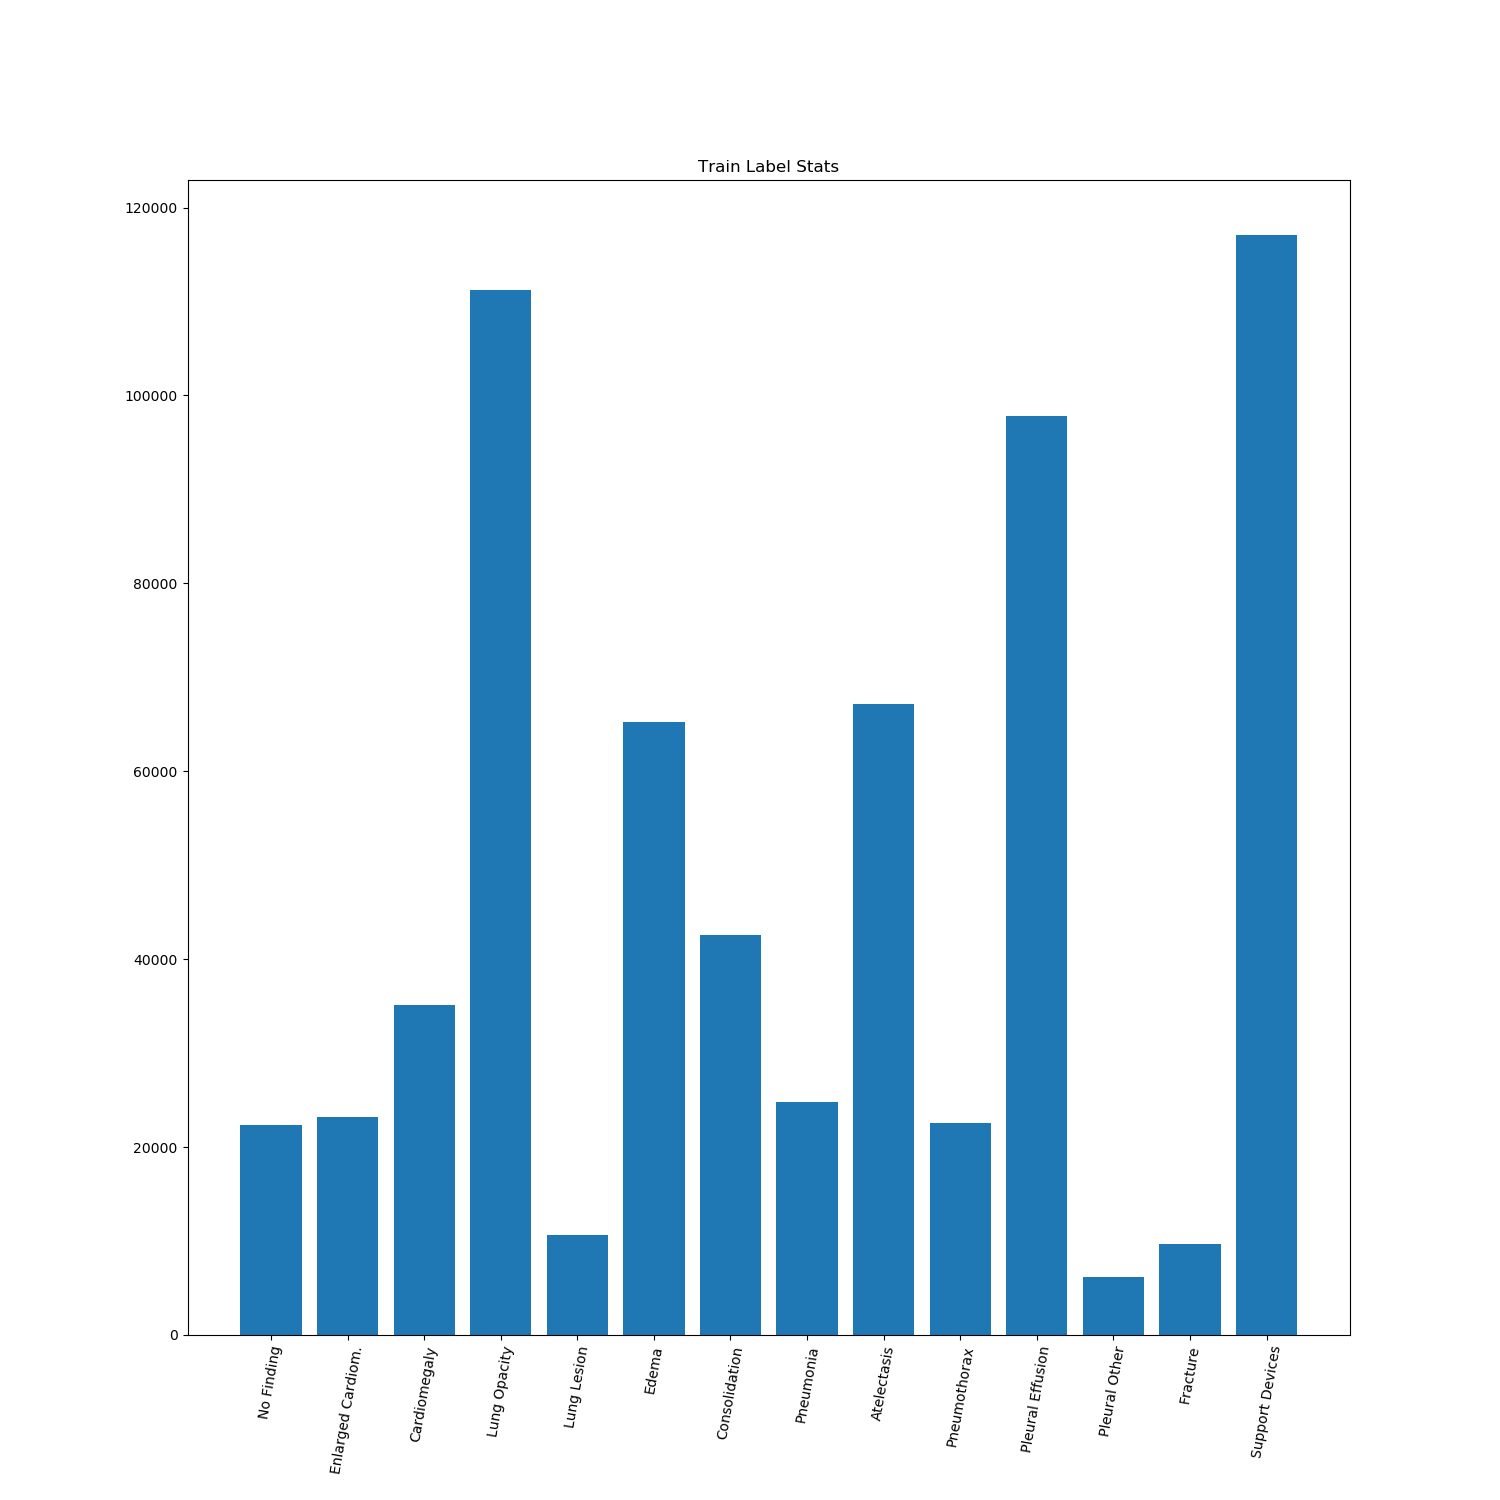
\includegraphics[width=\linewidth]{TrainLabelStats.png}
	\caption{Number of positive samples for each label in the training set}\label{fig:a}
\end{subfigure}
\begin{subfigure}{0.5\linewidth}
	\centering
	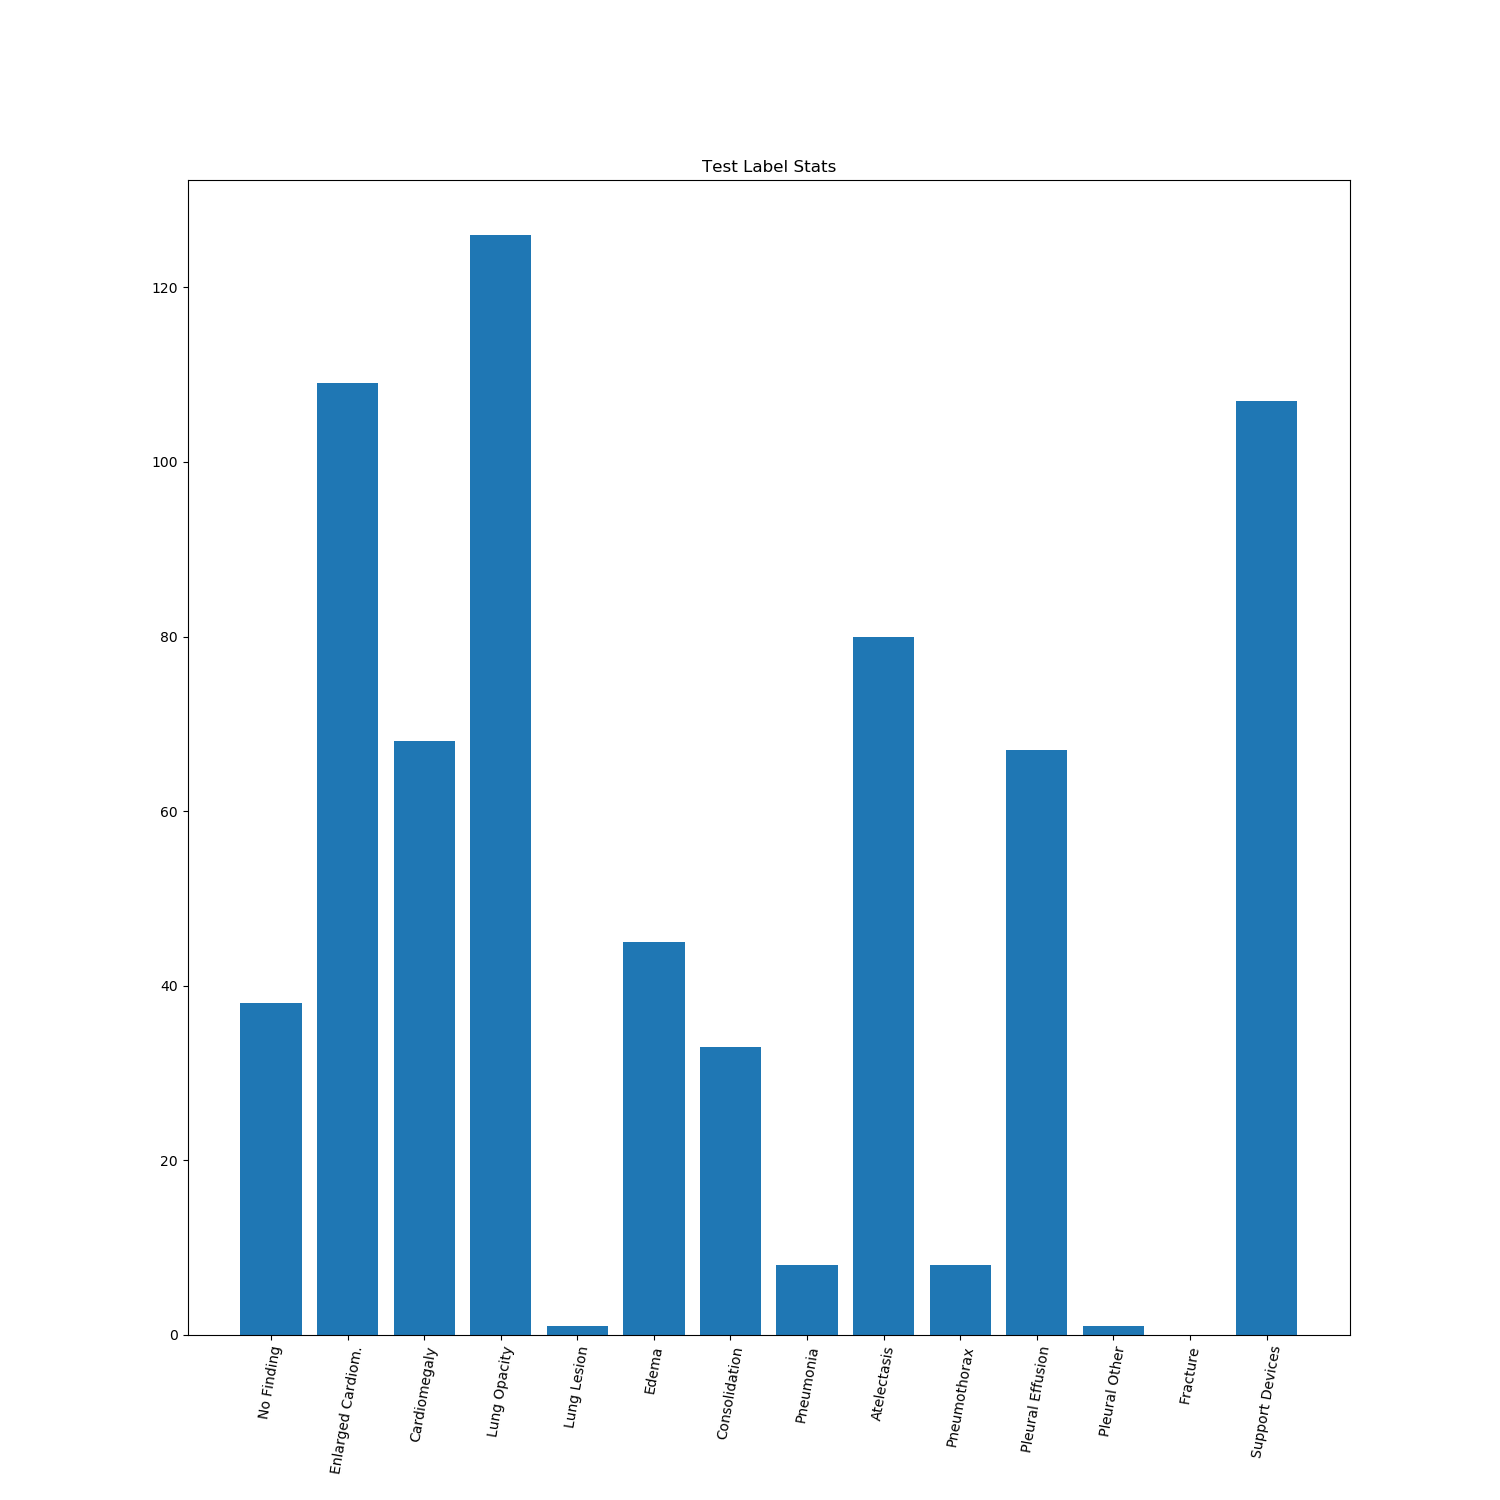
\includegraphics[width=\linewidth]{TestLabelStats.png}
	\caption{Number of positive samples for each label in the validation set}\label{fig:b}
\end{subfigure}
\caption{Positive label counts for all diseases}\label{label_counts}
\end{figure}

In Figure \ref{label_counts}, we list the numbers of positive samples for each label. As we can see with "Lung Lesion" and "Pleural Other", some labels have few samples in both the training and validation sets. This implies we need data augmentation to obtain balanced performance on all labels.

\section{Preprocessing}


The images can be classified according to the positioning of the patient into three classes: frontal-AP (anterposterior), frontal-PA (posterior-anterior), and lateral. This information may be useful for model tuning. We grouped the training set into these three classes. 

Each image is loaded into the RGB format and then is randomly horizontal flipped. Then the image is downsized and center-cropped to the size of $224\times224$. After the image is transformed into tensors, we normalized the tensors with $mean = [0.485, 0.456, 0.406]$ and $std = [0.229, 0.224, 0.225]$.

There are various ways to encode uncertainty values in the labels in the dataset, which are marked by -1. For simplicity we use U-Ones encoding in {\color{cyan}\cite{irvin}}. That is replacing -1 with 1. The reasoning is this kind of models are used to help human experts with the first-round screening. False negative is considered less preferable than false positive. Besides that we replace NaN with $0's$, turning missing values to negative values.


\section{Approach}

\subsection{Problem Formulation}
For each pathology, the detection task is a binary classification problem. We would like to optimize the \textit{binary cross entropy loss}, with default set-ups provided by PyTorch. For a single example in the training set, the binary cross entropy loss is

\[L(X, y ) = y\log p(y=1|X)+(1-y)\log p(y=0|X).\]


\subsection{Model Architecture}

We would like to reproduce CheXNet by  {\color{cyan}\cite{rajpurkar}} which is based on DenseNet-121 {\color{cyan}\cite{huang}}. DenseNets improve the flow of information and gradients through the network, making the optimization of very deep networks tractable. The structure of DenseNet-121 is shown in Figure \ref{DenseNet121}.


\begin{figure}[h]
	\centering
	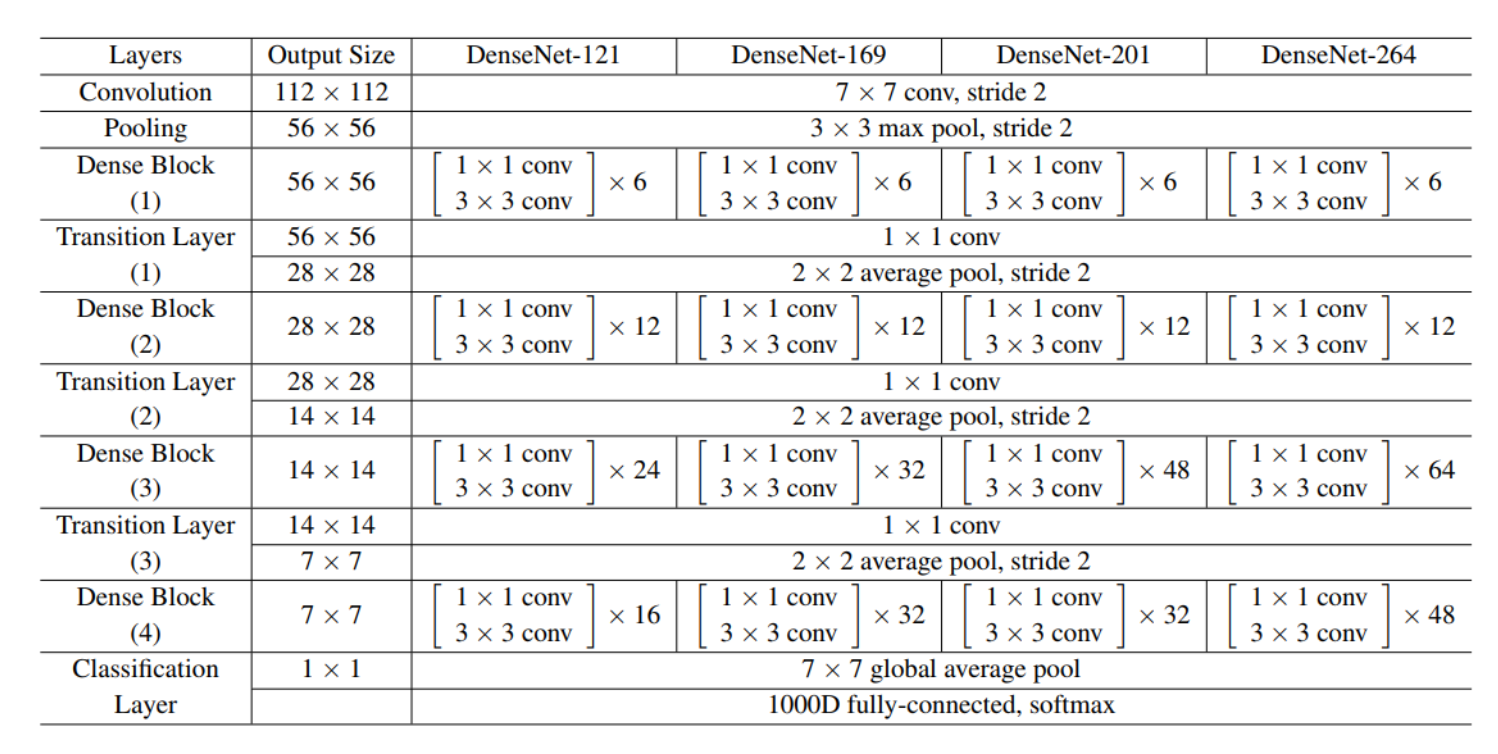
\includegraphics[width=0.8\linewidth]{densenet121.png}
	\caption{DenseNet-121}\label{DenseNet121}
\end{figure}


CheXNet replaces the final fully connected layer with one that has a single output, after which a sigmoid nonlinearity is applied. In the original paper {\color{cyan}\cite{rajpurkar}}, CheXNet is  trained on the ChestX-ray 14 dataset. However, here we will train the network on the bigger dataset CheXpert. 



\subsection{Implementation and Training Environment}



Our implementation is written in Python. Due to the large size of the dataset,  we choose to use PyTorch and Keras to utilize GPU to accelerate the training process. We initialized the model with the pre-trained DenseNet121 provided in PyTorch. We used the Adam with $\beta_1 = 0.9$, $\beta_2 = 0.999$, and learning rate $0.0002$ to train our model, which are identical to the values used in {\color{cyan}\cite{irvin}}.

The model was trained on a desktop with an i5-3470 CPU, 16 GB RAM and a GTX 1070 GPU with 8 GB on-board memory. The GPU supports single-precision floating-point number training only. The number of trainable parameters in DenseNet121 is close to 7 million. During training, back-propagation can take up to 3 times of the size of the memory required by forward-propagation. Given \texttt{batch\_size} $=32$, the parameters alone can take $7000000 \times 4 \times 32 \div 1024 \div 1024 \times 3 = 2563$ MB memory. The remaining overhead is largely implementation-dependent. Through trial and error, we found that mini-batches of size 64 could not be fit into 8 GB on-board memory, so we opted for \texttt{batch\_size} $=32$.


We use AUROC to evaluate the performance of the model.

\subsection{Training Procedure and Pitfalls}
With the given model architecture, we tried three different approaches and used AUROC to evaluate the resulting models.


First we tried training the model from scratch, given that the model was loaded with pre-trained weights on ImageNet dataset. Then we save the model and generated the AUROC data for each of the pathologies.

In this approach, we implemented the procedure in PyTorch. Before feeding data to the model, we randomly flip the data as a way of doing data augmentation. We also resized the images to $224 \times 224$ so that the size matched the input size of the model. We also did standardization to the images. We trained the model for 5 epochs, each epoch took 6981 batches and each batch contained 32 images.

In the second approach, we tried \textit{transfer-learning}. We first load the base model and adapted it to the customized form as we mentioned before. Then we froze the layers that were not customized by us, which had the weights trained on ImageNet dataset. The only layer that was trainable was the last classification layer we added to the model, which was initialized randomly.

The data preprocessing step was done slightly differently in this approach. We just resized the images to $224 \times 224$ and shift all pixel values to the range between 0 and 1. Other than that everything else including parameter values and training steps was the same as the first approach.


We implemented the procedure in Keras and trained it for 3 epochs. Because only the last layer was trainable, the bottleneck during the training was the image loading to GPU and GPU was idle from time to time.

In the third approach we continued training based on the model we obtained from the second approach. In theory, this can avoid the flaw in the first approach. That is when some of the layers have fine-tuned weights and others have random weights, the gradients generated and propagated by the random weights tend to be too large to overtune the fine-tuned weights, cause the model to take longer time to converge.

The data preprocessing and training steps were the same as the second approach. We trained for 3 epochs. This time the GPU became the bottleneck of the training.

In all three approaches we saved the best checkpoint based on some metric. In the first approach we used validation loss as the metric while in the second and third ones we used validation accuracy as the metric.

\begin{figure}
\begin{subfigure}{0.33\linewidth}
	\centering
	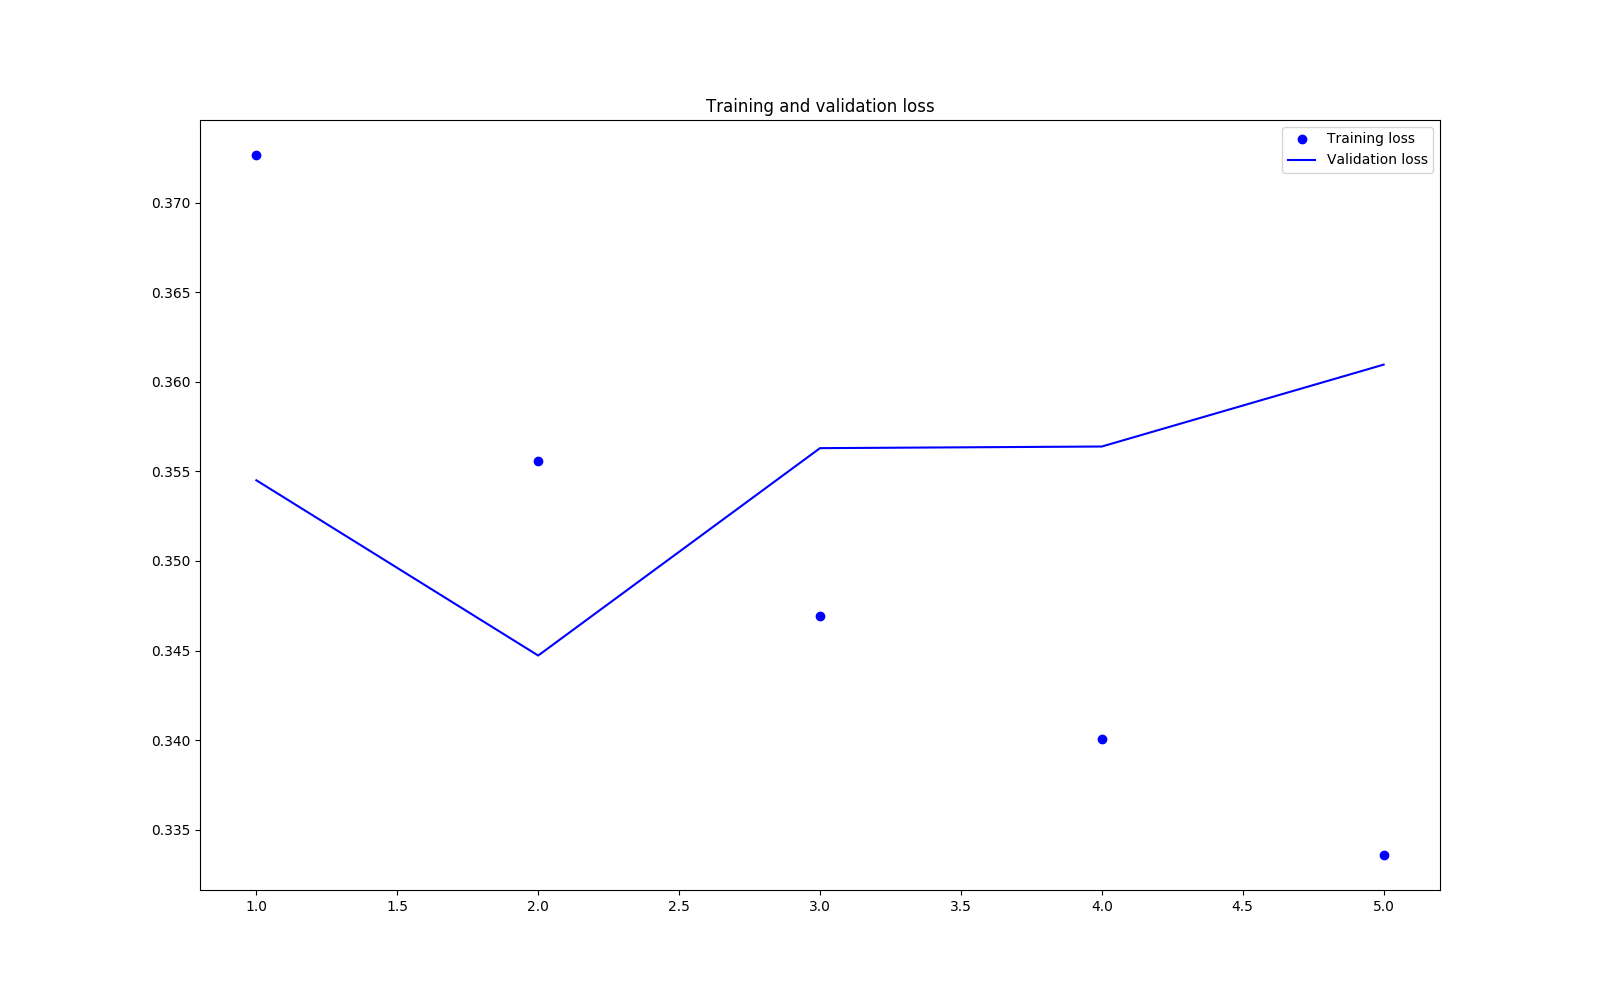
\includegraphics[width=\linewidth]{train_val_loss_plot.png}
	\caption{First approach, training and validation loss}  \label{fig:a}
\end{subfigure}
\begin{subfigure}{0.33\linewidth}
	\centering
	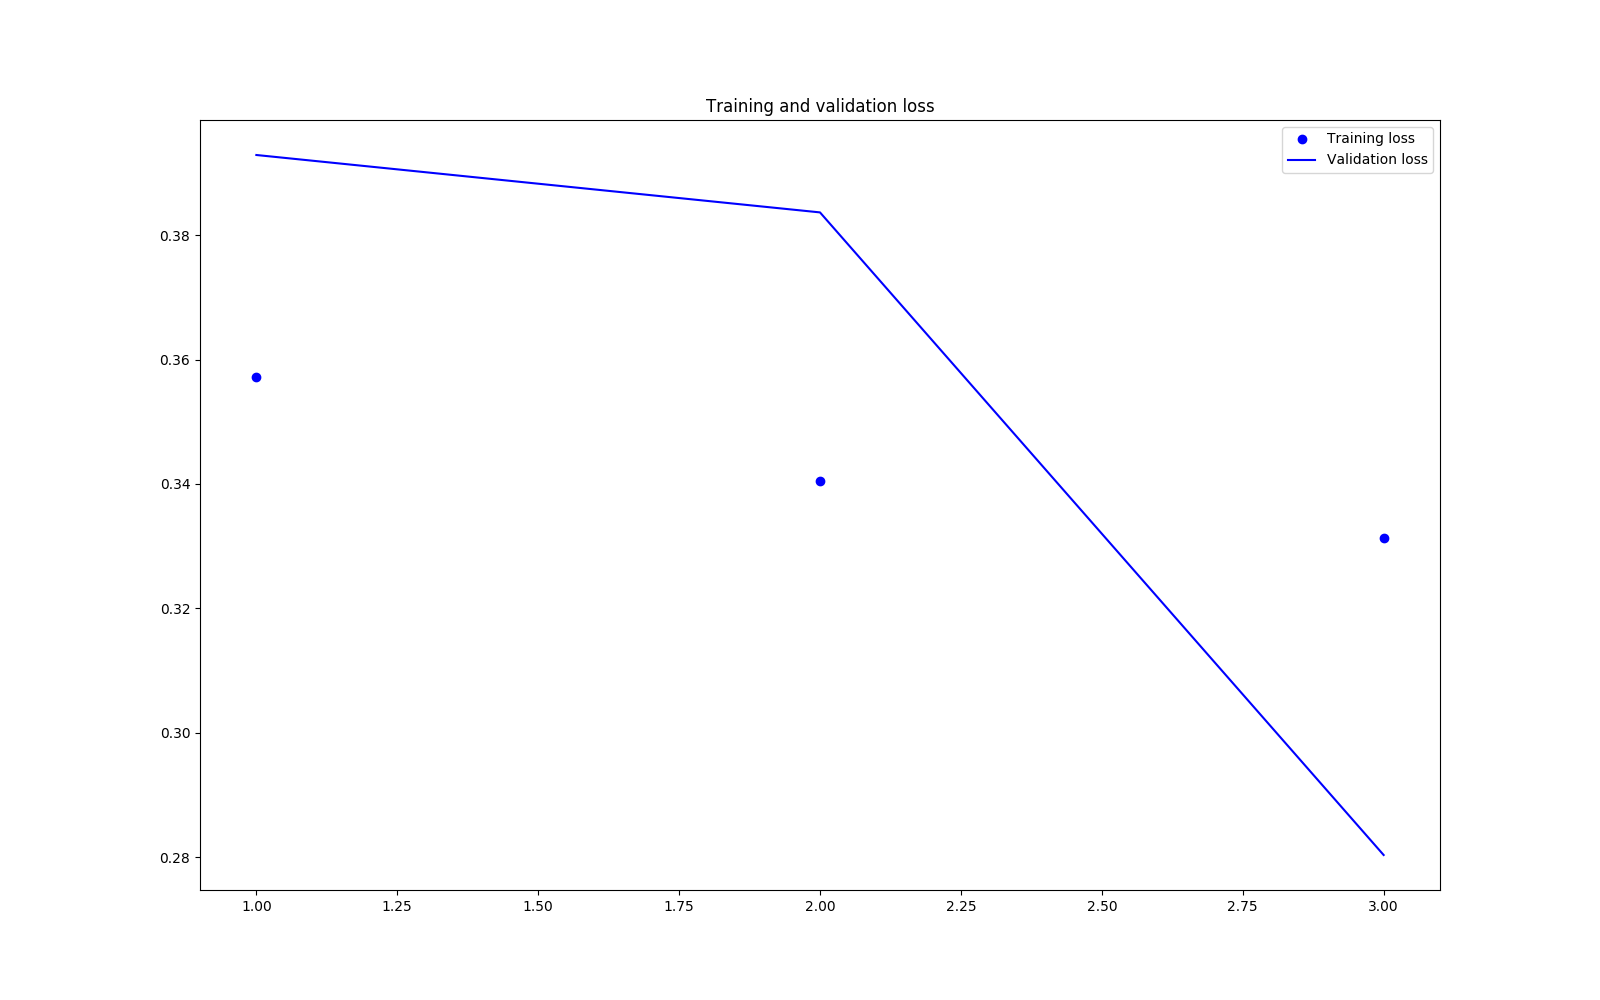
\includegraphics[width=\linewidth]{chexpert_keras_tf_to_full_loss.png}
	\caption{Second approach, training and validation loss}  \label{fig:b}
\end{subfigure}
\begin{subfigure}{0.33\linewidth}
	\centering
	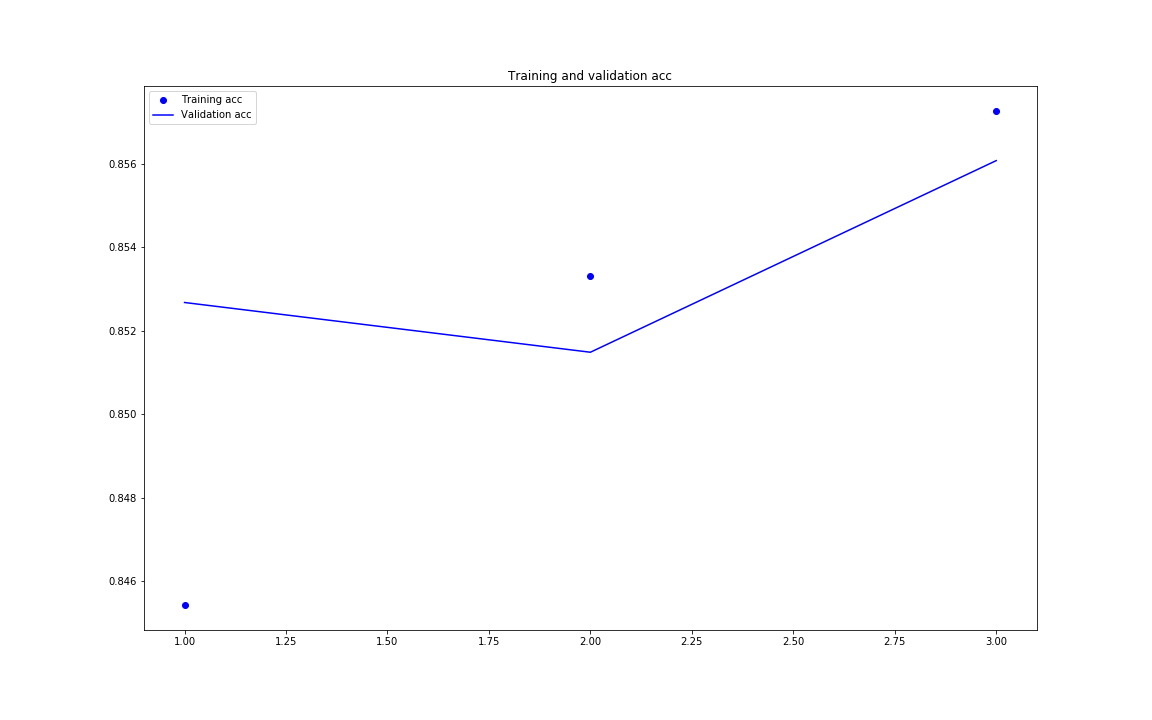
\includegraphics[width=\linewidth]{chexpert121_acc_tf_to_full.png}
	\caption{Third approach, training and validation accuracy}  \label{fig:c}
\end{subfigure}
\caption{Selective training plots}\label{train_plots}
\end{figure}

In Figure \ref{train_plots} we present some of the plots we collected during training the model using the three approaches.


While building the model we have difficulty to understand how different libraries constructed the base model DenseNet121. In Keras, the single layers are encapsulated in blocks, which are essentially custom layers. By removing the last classification layer we actually removed the last fully connected layer and the global average pooling layer. To keep the model the same as the one used in {\color{cyan}\cite{rajpurkar}} we carefully added back the pooling layer.


But in PyTorch things are done differently. When we looked into the structure of DenseNet121 in PyTorch we did not find the last global pooling layer. It turned out to be the case that for layers without trainable parameters one could use static layers provided in a particular package in PyTorch. This kind of layers are not visible by printing the model or using third party visualization tools. We found out by looking into the PyTorch source code.

We used to train as many as 20 epochs to see how much time did it take the training to overfit the model. It turned out to be that after 5 epochs the gap between training and validation loss increased monotonically. Later we adjusted it to 5 or fewer epochs to save time. This is validated by the number of epochs used by authors of different papers we cite.

\section{Experimental Results}

The AUROC scores of our model on the five selected pathology are in Table \ref{AUROC}. Those are the diseases presented in {\color{cyan}\cite{irvin}}


\begin{table}[th]
	\centering
	\begin{tabular}{ | c | c | c | c | c | }
		\hline
		Pathology & Transfer Learning & Trained from Scratch & Trained from TF & CheXpert \\
		\hline
		Atelectasis & 0.720 & 0.834 & 0.788 & 0.858 \\
		\hline
		Cardiomegaly & 0.673 & 0.790 & 0.831 & 0.832 \\
		\hline
		Consolidation & 0.658 & 0.868 & 0.857 & 0.899 \\
		\hline
		Edema & 0.779 & 0.906 & 0.911 & 0.941 \\
		\hline
		Pleural Effusion & 0.724 & 0.920 & 0.933 & 0.934 \\
		\hline
	\end{tabular}
	\caption{AUROC Scores: All models are compared under U-Ones encoding}\label{AUROC}
\end{table}

In Figure \ref{auroc} we show the AUROC curves for the five listed diseases collected from the model trained directly from scratch.

\begin{figure}[th]
\begin{subfigure}{0.19\linewidth}
	\centering
	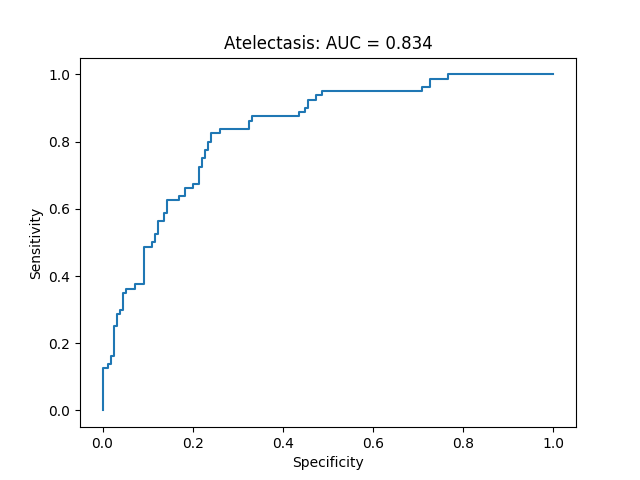
\includegraphics[width=\linewidth]{Atelectasis_roc.png}
	\caption{Atelectasis}\label{ROC_Atelectasis}
\end{subfigure}
\begin{subfigure}{0.19\linewidth}
	\centering
	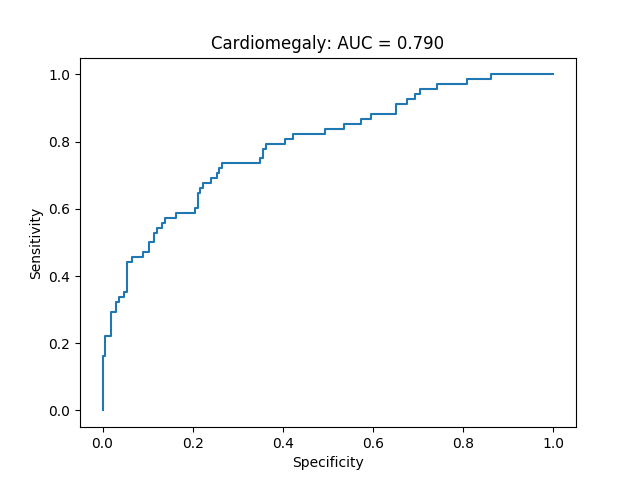
\includegraphics[width=\linewidth]{Cardiomegaly_roc.png}
	\caption{Cardiomegaly}\label{ROC_Cardiomegaly}
\end{subfigure}
\begin{subfigure}{0.19\linewidth}
	\centering
	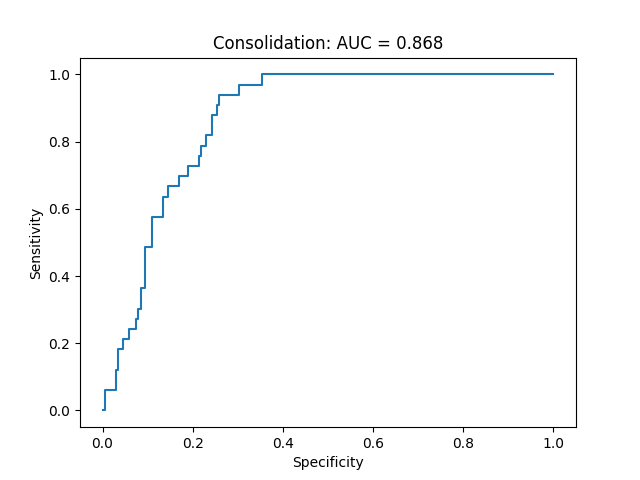
\includegraphics[width=\linewidth]{Consolidation_roc.png}
	\caption{Consolidation}\label{ROC_Consolidation}
\end{subfigure}
\begin{subfigure}{0.19\linewidth}
	\centering
	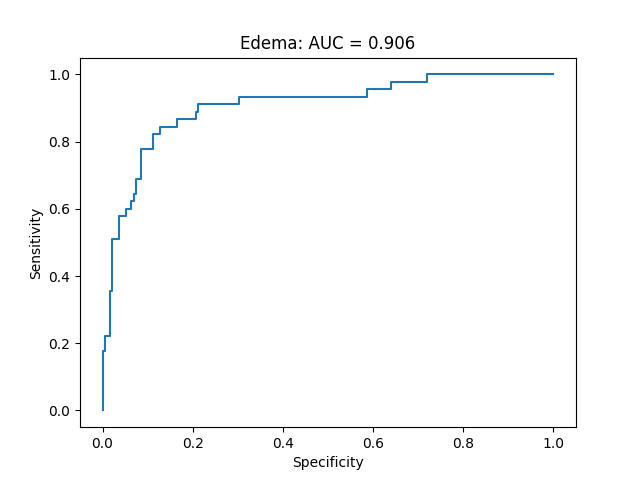
\includegraphics[width=\linewidth]{Edema_roc.png}
	\caption{Edema}\label{ROC_Edema}
\end{subfigure}
\begin{subfigure}{0.19\linewidth}
	\centering
	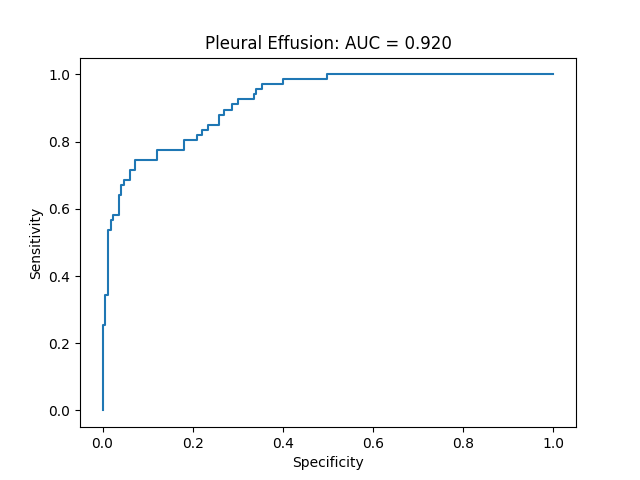
\includegraphics[width=\linewidth]{Pleural_Effusion_roc.png}
	\caption{Pleural Effusion}\label{ROC_Pleural_Effusion}
\end{subfigure}
\caption{AUROC curves for selected diseases from trained from scratch model}\label{auroc}
\end{figure}


As we can see, transfer learning based on the pre-trained model produced a model that is not competitive. In general transfer learning is suitable for situations where data for the interested task is hard to get. For those scenarios transfer learning can produce robust models with very few data. Also it takes little time to train. In our case, the available training images are over two hundred thousand which is not the best case to apply transfer learning.


The other two approaches produced models with similar performance in terms of AUROC. In training from scratch, we did more data augmentation steps. It did not bring noticeable advantage over the model trained on transfer learned one. It could be that we need more aggressive data augmentation which would take more time to train.

On average, the transfer learner based model slightly outperforms the one trained from scratch. It is difficult to tell if the third approach is truly effective in this scenario because their performance are close to each other.

\begin{figure}[ht]
\begin{subfigure}{0.5\linewidth}
	\centering
	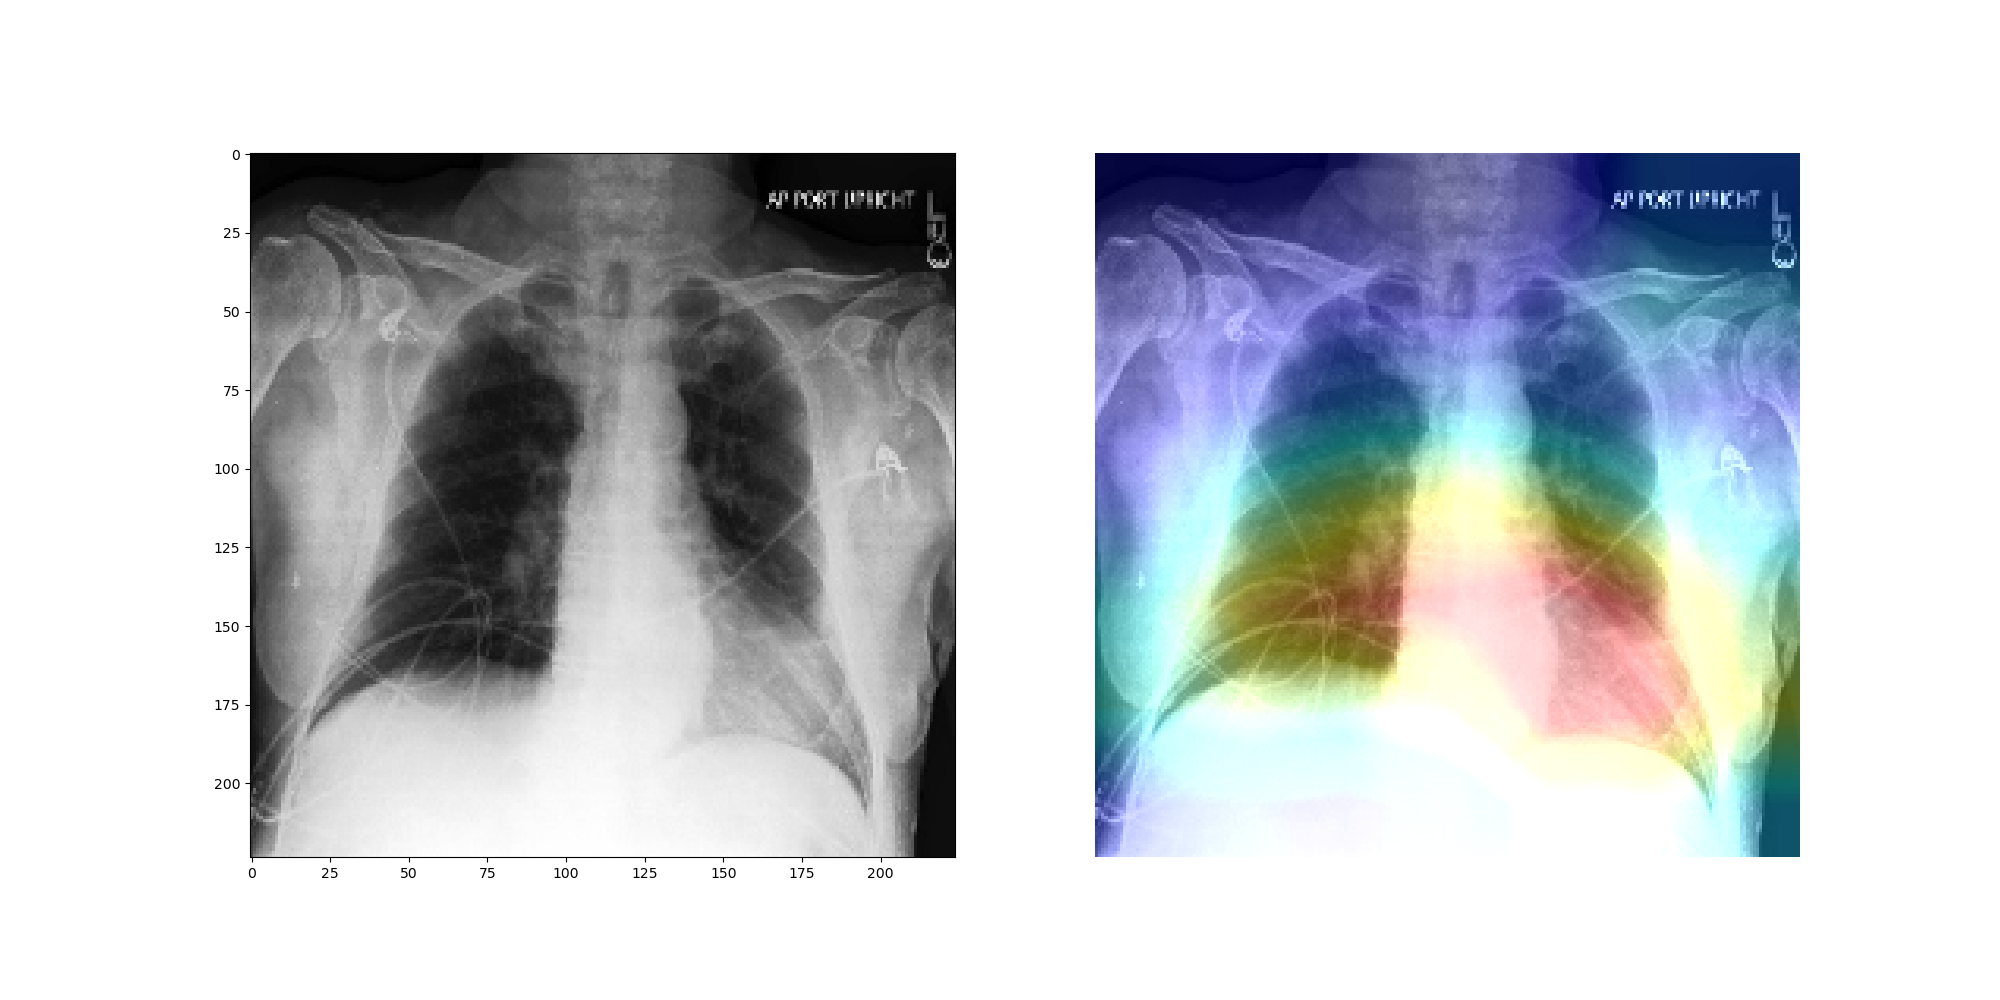
\includegraphics[width=\linewidth]{patient64541_1.png}
	\label{fig:a}
\end{subfigure}
\begin{subfigure}{0.5\linewidth}
	\centering
	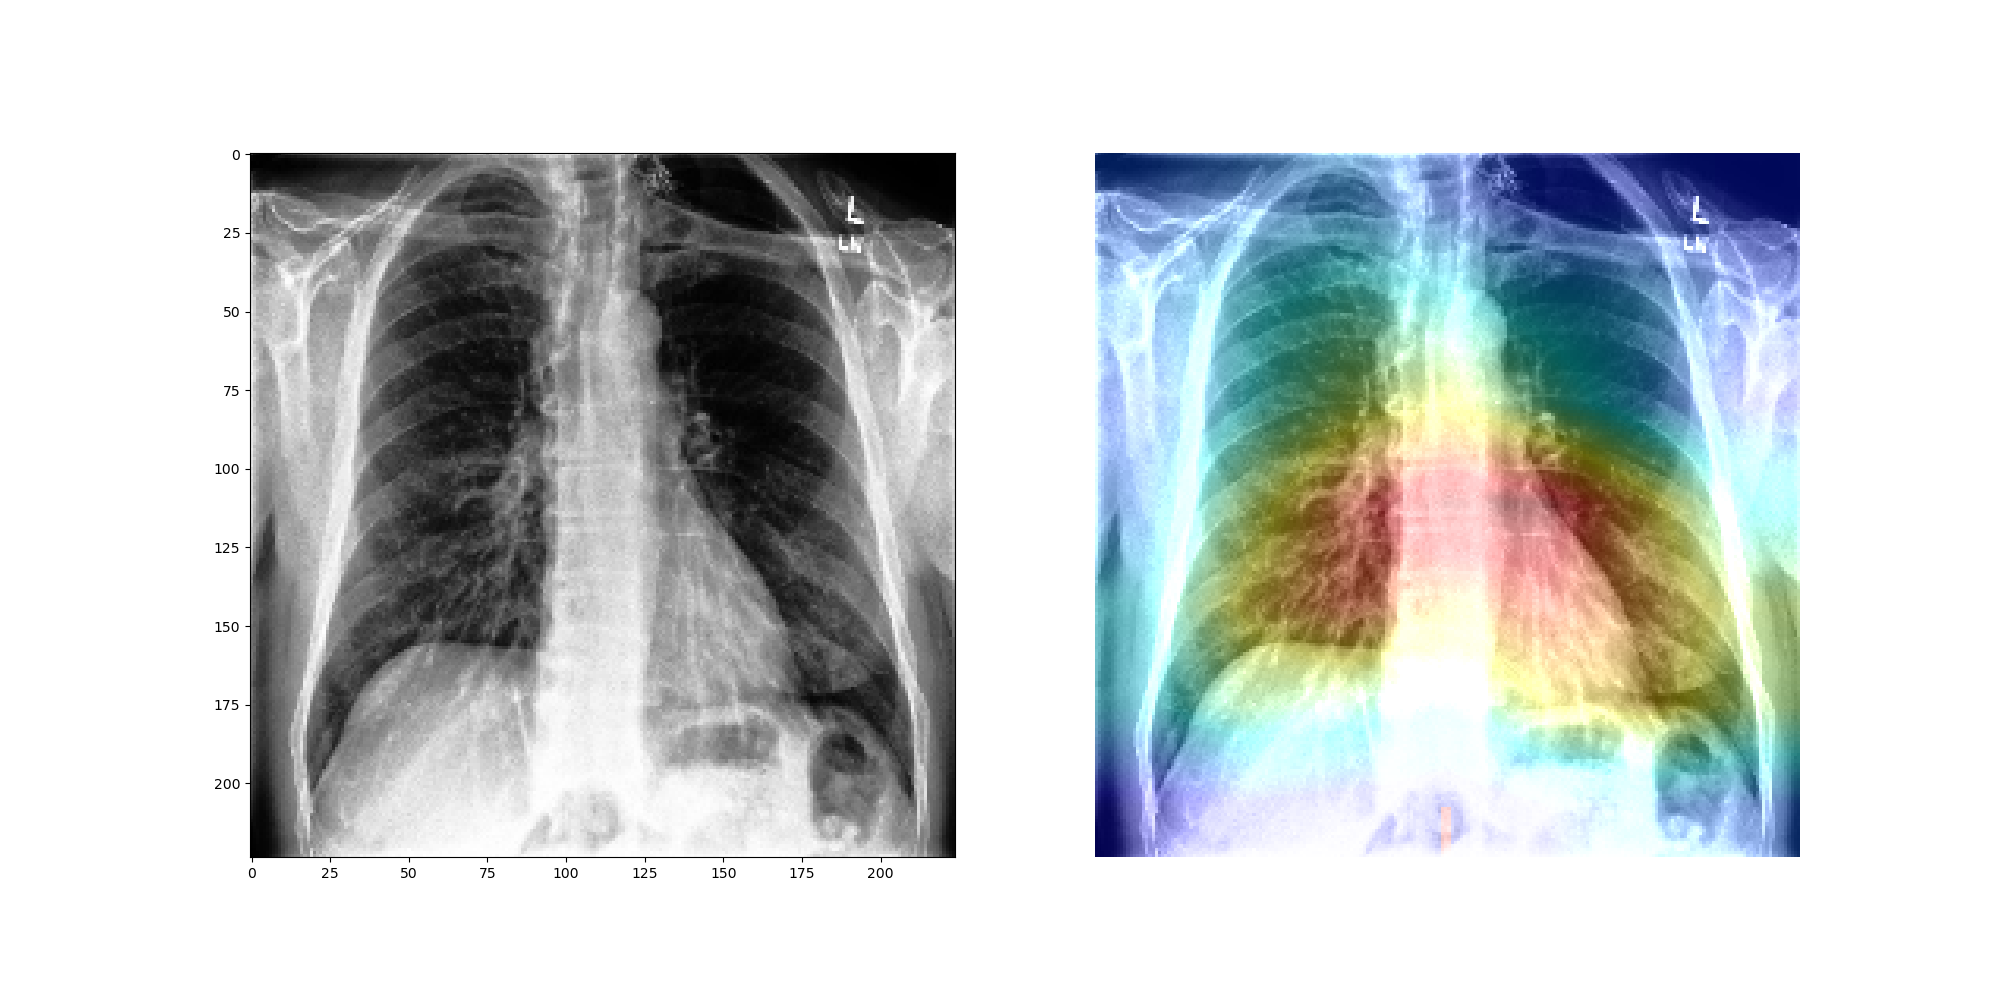
\includegraphics[width=\linewidth]{patient64547_1.png}
	\label{fig:b}
\end{subfigure}
\par\bigskip
\begin{subfigure}{0.5\linewidth}
	\centering
	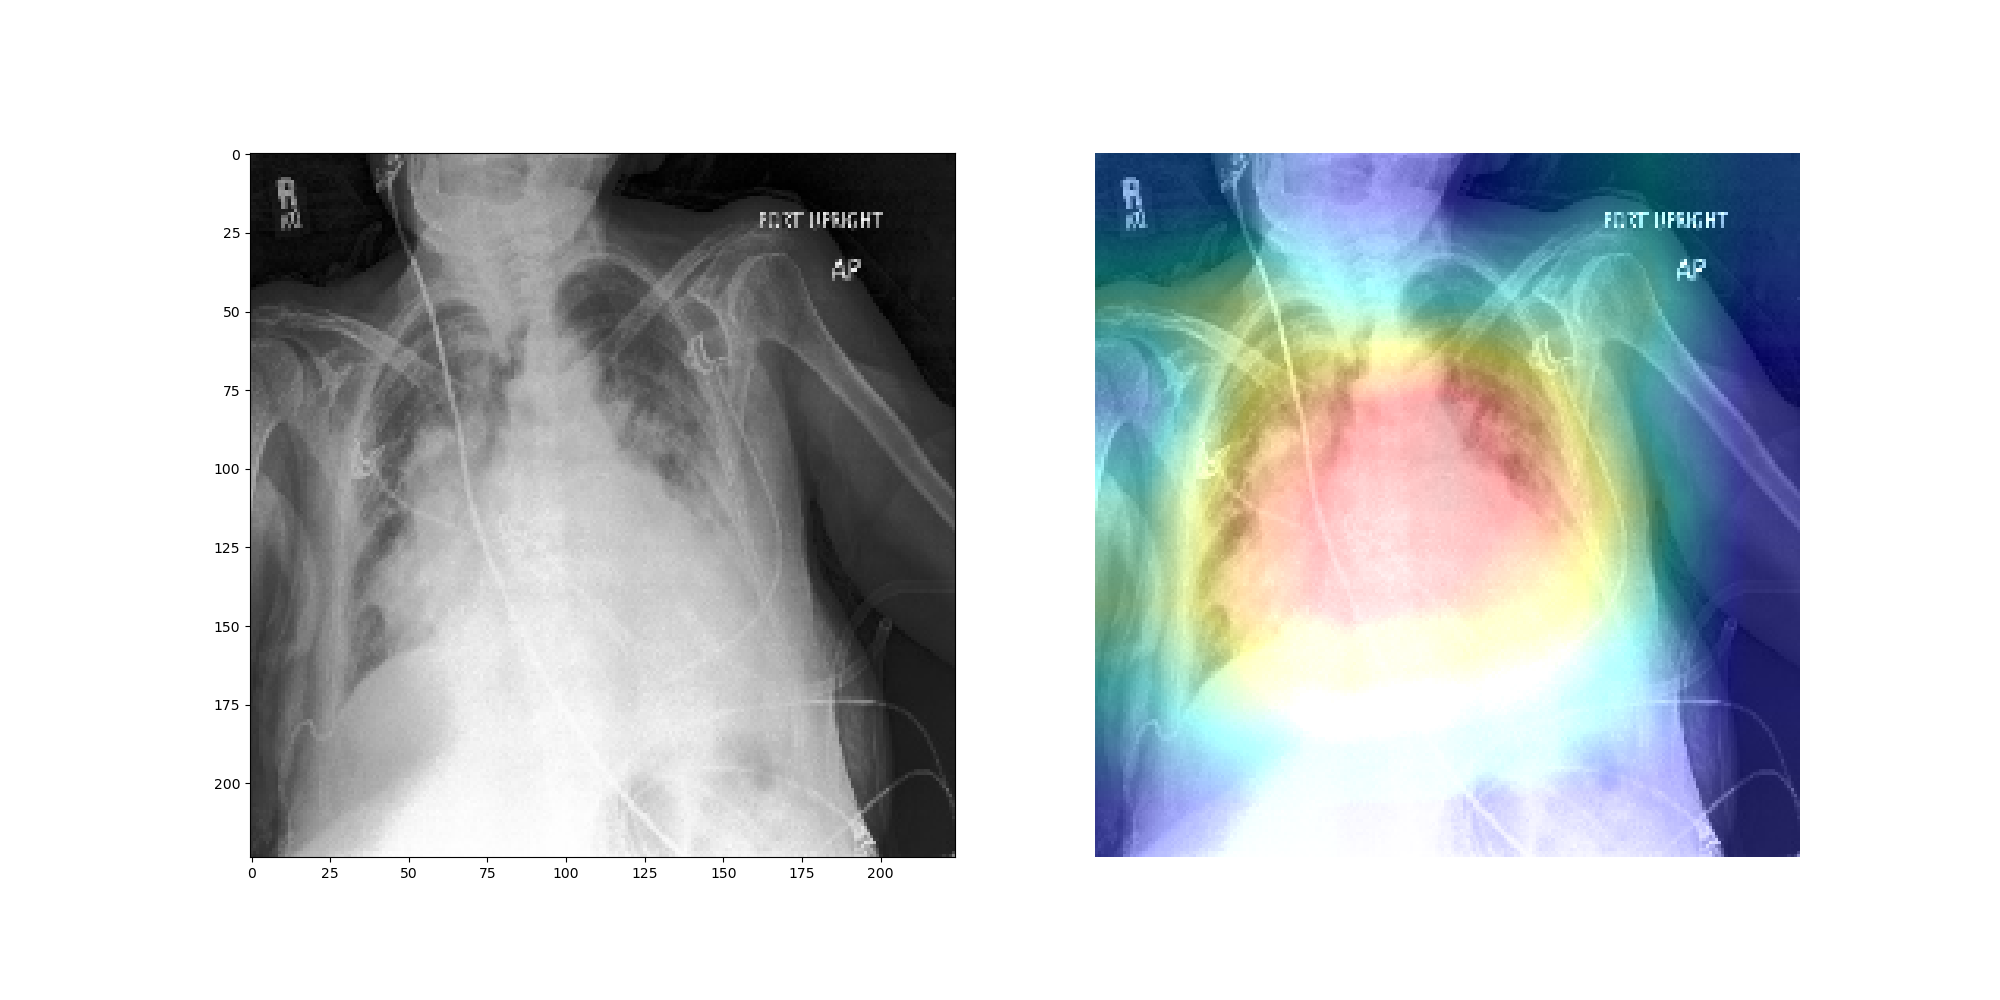
\includegraphics[width=\linewidth]{patient64552_1.png}
	\label{fig:c}
\end{subfigure}
\begin{subfigure}{0.5\linewidth}
	\centering
	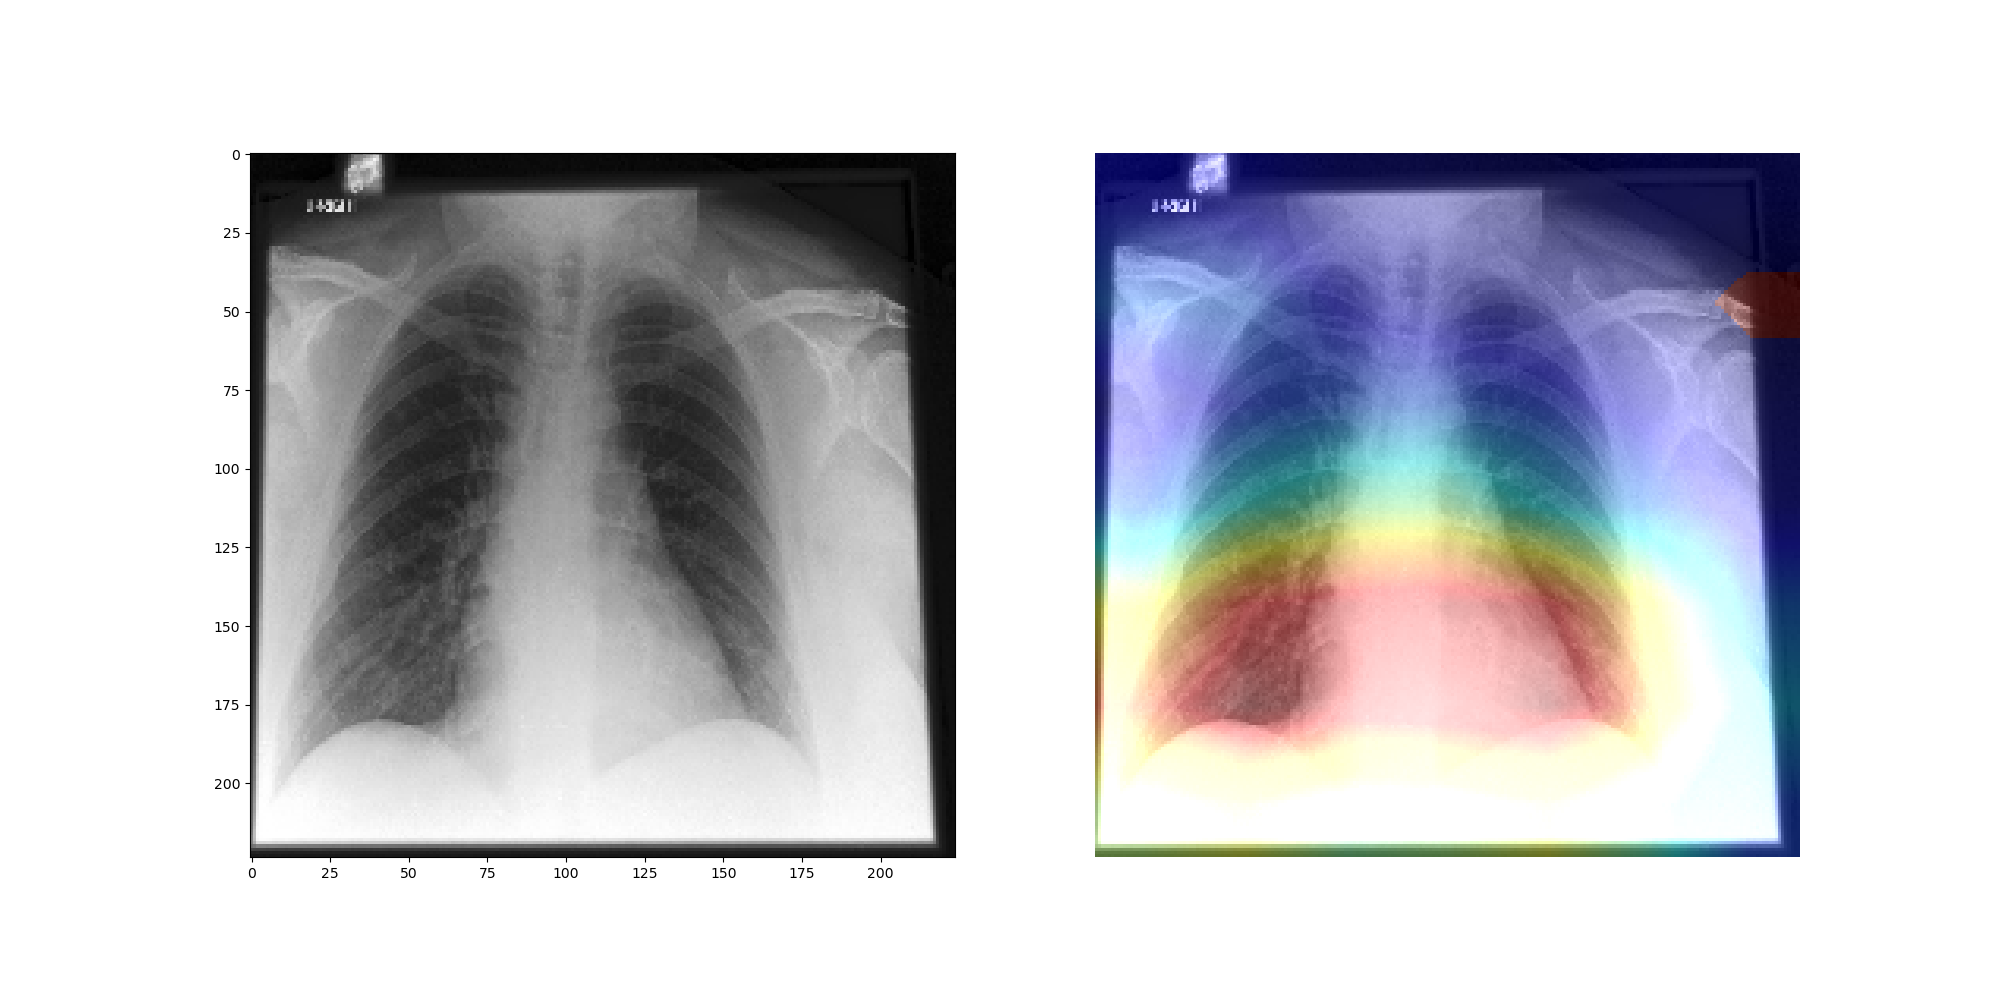
\includegraphics[width=\linewidth]{patient64739_1.png}
	\label{fig:d}
\end{subfigure}
\caption{Our model localizes findings in images via Gradient-based localization.}
\end{figure}

We applied \textit{class activation map} technique to the raw images and found that it performed well localizing the lesion. We used the same implementation employed by {\color{cyan}\cite{irvin}}, which was proposed by {\color{cyan}\cite{Selvaraju}}.

\section{Discussion}


With the same label encoding U-Ones two of our trained models achieved performance that is comparable to the one presented in {\color{cyan}\cite{irvin}}.


In {\color{cyan}\cite{irvin}} the model is the ensemble of 30 checkpoints from 3 epochs. The checkpoints are the best 10 checkpoints from each of the 3 epochs. Checkpoints are saved every 4800 batches. Batch size is 16.

From the performance of our models on labels "Atelectasis" and "Cardiomegaly" we can see that ensemble of our best two models might be beneficial. If we ensembled the checkpoints from the training we might get even better performance.

\begin{figure}[h]
	\centering
	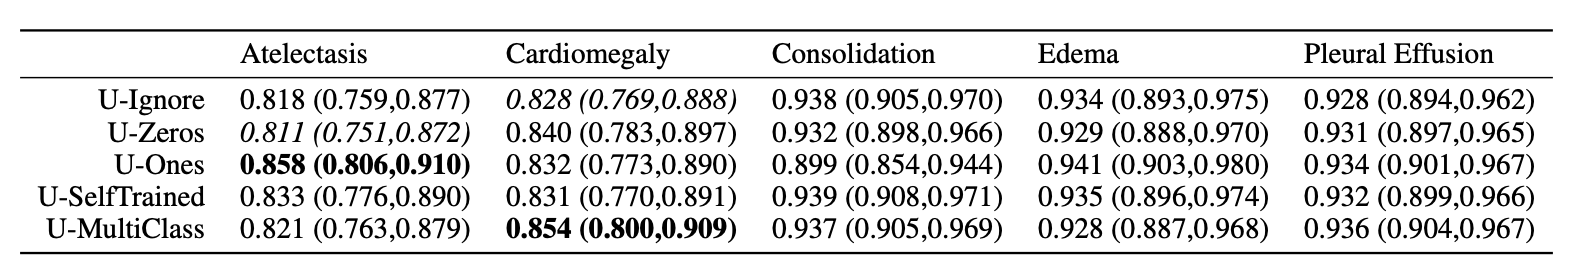
\includegraphics[width=1\linewidth]{CheXPert_results.png}
	\caption{Results Obtained in {\color{cyan}\cite{irvin}}}\label{CheXPert_results}
\end{figure}

Figure \ref{CheXPert_results} shows the AUROC values for the selected diseases by the ensemble models using different label encodings. Note that even our coarse single model outperforms all the ensemble models using encodings other than U-Ones in "Atelectasis". This validates the experimental results in {\color{cyan}\cite{irvin}}.

Another thing we may learn from Figure \ref{CheXPert_results} is different encodings perform differently for different labels. Thus we can encode data with more than one encoding strategies. For example, for the label column that corresponds to "Atelectasis" we may encode the data with U-Ones and for the label column that corresponds to "Cardiomegaly" we may encode the data with U-MultiClass.

\section{Conclusion}

We implemented the CheXNet and trained it using the CheXpert dataset. The overall performance of our model is on par with the ones proposed in the original paper.

There are a few techniques that we could apply to the model to potentially improve the model performance but did not due to time constraints.
\begin{itemize}
	\item Ensemble
	\item Aggressive data augmentation
	\item Mixed label encoding
\end{itemize}

Despite that we did not apply all the techniques that we were aware of, we were able to achieve results that were close to the state of the art research using a single model.

\section{Team Contributions}

\textbf{Xiao-Hong Deng:} Improved PyTorch model. Implemented Keras models. Trained and tuned all the models. Implemented some io and visualization code to help with the training and analysis. Contributed Dataset and Approach sections in the proposal and was responsible for organizing and putting sections from all team members together to form the final proposal. Wrote the final report based on the draft.


\textbf{Gerry Meixiong:} Integrated the CheXPert dataset for use with PyTorch, including data transformations and pre-processing. Added functionality to train and test a PyTorch model, including calculating and plotting AUROC. Responsible for the Project Presentation.

\textbf{Chenxu Wen:} Worked with Lan Yao to implement the main PyTorch model of the project. Implemented the  gradient-based heatmap for the model . Wrote an initial version of the project proposal. Wrote the project draft based on results on the first iteration.

\textbf{Lan Yao:} Implemented the code that generates the label distribution graph. Implemented the PyTorch model and the training process used in our first approach. Hook up the heatmap generation code with the main program to generate the heatmap graphs used in the paper. Wrote a version of project proposal and mainly contributed the Related Work section to the final proposal.

\small
\bibliographystyle{apalike}
\bibliography{ref}


\end{document}

